\section{Einleitung} % (fold)
\label{sec:einleitung}

	Durch die Wechselwirkung einer Lichtwelle mit den Elektronen der Materie werden die Ausbreitungsgeschwindigkeiten $v$ des Lichtes kleiner als die Vakuumlichtgeschwindigkeit $c$.
	Es wird sich herausstellen, dass die Geschwindigkeit von der Wellenl"ange des Lichtes abh"angt. Dieses Ph"anomen wird als Dispersion bezeichnet.
	
\section{Theorie} % (fold)
\label{sec:theorie}

	\subsection{Brechung, Brechungsindex und Dispersionskurve} % (fold)
	\label{sub:brechungsindex}
	
	Tritt ein Lichtstrahl schr"ag in Materie ein, so erf"ahrt er durch die "Anderung der Geschwindigkeit an der Grenzfl"ache eine Richtungs"anderung.

	Dies wird als Brechung bezeichnet und wird durch den Brechungsindex $n$ beschrieben.

	Dieser ist definiert durch das Verh"altnis der beiden Lichtgeschwindigkeiten.

	\begin{equation}
		n := \frac{v_\mathrm{1}}{v_\mathrm{2}}  \label{gl:brechung}
	\end{equation}

	F"ur die Ausbreitungsgeschwindigkeit gilt:

	\begin{equation}
		v = \lambda \frac{\omega}{2\pi}
	\end{equation}

	Daraus folgt, dass auch der Brechungsindex $n$ eine frequenzabh"angige bzw.	wellenl"angenabh"angige Gr"o"se ist und somit eine Funktion im Bereich des sichtbaren Lichtes.

	Dies wird als Dispersionskurve bezeichnet.

	\begin{equation}
		n = f(\lambda) 
	\end{equation}

	\subsection{Das Huygenssche Prinzip} % (fold)
	\label{sub:das_huygenssche_prinzip}
	
	\begin{figure}[!h]
		\centering
		\includegraphics[width = 8cm]{img/huygen.jpg}
		\caption{Das Huygens'sche Prinzip und die daraus resultierenden wichtigen Gr"o"sen f"ur die Herleitung des Snelliusschen Brechungsgesetzes, \cite{anleitung}}
		\label{huygen}
	\end{figure}

	Jeder Punkt einer bestehenden Wellenfl"ache kann als Zentrum einer neuen kugelf"ormigen "`Elementarwelle"' aufgefasst werden. Die Einh"ullende aller Elementarwellen gibt die Wellenfront f"ur einen sp"ateren Zeitpunkt. Durch die Geschwindigkeits"anderung an einer Grenzfl"ache kommt so eine Richtungs"anderung zustande (Abb. \ref{huygen}).

	In der Zeit T = $\bar{BC}$/$v_\mathrm{1}$ erreicht der Punkt B die Grenzfl"ache. In der Zeit hat die Welle im Punkt A jedoch bereits die Strecke T$v_\mathrm{2}$ =  $\bar{AA'}$ zur"uckgelegt. Wird dies "uber die Winkel in Beziehung gesetzt, so ergibt sich:

	\begin{equation}
		\frac{\sin(\alpha)}{\sin(\beta)} = \frac{v_\mathrm{1}}{v_\mathrm{2}}  \label{gl:huygen}
	\end{equation}

	Aus Gleichung \eqref{gl:brechung} ergibt sich damit das Snelliussche Brechungsgesetz:

	\begin{equation}
		\frac{\sin(\alpha)}{\sin(\beta)} = n  \label{snellius}
	\end{equation}

	\subsection{Dispersionsgleichung} % (fold)
	\label{sub:dispersionsgleichung}
	
	Wie bereits in Kapitel \ref{sub:brechungsindex} festgestellt wurde, ist der Brechungsindex von der Freuquenz bzw. der Wellenl"ange des Lichts abh"angig. Dies wird als Dispersion bezeichnet. Die Dispersionskurve eines Materials ist von Interesse, da durch Kombination unterschiedlicher Linsen mit verschiedenen Dispersionskurven die chromatische Aberration zu kompensieren ist.

	Es wird nun die Dispersionsgleichung hergeleitet.
	Um ein g"ultiges Modell benutzen zu k"onnen, ohne auf die Quantentheorie zur"uckgreifen zu m"ussen, darf Licht und Materie nicht in Resonanz miteinander treten k"onnen.
	Dies ist bei Gl"asern im sichtbaren Spektralbereich gegeben.
	Tritt eine ebene Lichtwelle mit der elektrischen Feldst"arke 

	\begin{equation}
		\vec{E} = \vec{E_\mathrm{0}} \exp{(i \omega t)}
	\end{equation}

	auf ein Materiel, so wirkt dadurch eine periodische Kraft

	\begin{equation}
		\vec{F_\mathrm{e}} = q_\mathrm{h} \vec{E}
	\end{equation}

	auf die Ladung $q_\mathrm{h}$.
	Zudem wirkt der Auslenkung der Ladungstr"ager eine r"ucktreibende Kraft $\vec{F_\mathrm{r}}$ entgegen, welche proportional zur Auslenkung ist. Weiterhin wirkt auf die periodische Bewegung der Teilchen eine Art Reibungskraft $\vec{F_\mathrm{d}}$ proportional zur Geschwindingkeit.
	Es ergibt sich hieraus eine DGL f"ur $x_\mathrm{h}$. Diese wird mit $N_\mathrm{h} q_\mathrm{h} / m_\mathrm{h}$ erweitert um diese durch die Polarisation $\vec{P_\mathrm{h}}$ auszudr"ucken. 

	Es ergibt sich:

	\begin{equation}
		\frac{\mathrm{d}^2 \vec{P_\mathrm{h}}}{\mathrm{d} t^2} + \frac{f_\mathrm{h}}{m_\mathrm{h}} \frac{\mathrm{d} \vec{P_\mathrm{h}}}{\mathrm{d} t} + \frac{a_\mathrm{h}}{m_\mathrm{h}} \vec{P_\mathrm{h}} = \frac{N_\mathrm{q} {q_\mathrm{h}}^2}{m_\mathrm{h}} \vec{E_\mathrm{0}} \exp{(i \omega t)} 
	\end{equation}

	Dies ist die bekannte DGL f"ur eine erzwungene Schwingung. Die L"osung lautet:

	\begin{equation}
		\vec{P_\mathrm{h}} = \frac{1}{{\omega_\mathrm{h}}^2 - w^2 + i \frac{f_\mathrm{h}}{m\mathrm{h}} \omega} \frac{N_\mathrm{h} {q_\mathrm{h}}^2}{m_\mathrm{h}} \vec{E_\mathrm{0}} \exp{(i \omega t)} 
	\end{equation}

	Nun muss noch "uber alle h summiert werden um die gesamte Polarisation zu erhalten. Benutzt man nun, dass $\vec{P} = (\epsilon - 1) \epsilon_\mathrm{0} \vec{E}$  ist und $n^2 = \epsilon$ erh"alt ergibt sich ein Zusammenhang zwischen dem Brechungsindex und der Frequenz bzw. der Wellenl"ange.
	Es folgt:

	\begin{equation}
		\tilde{n}^2 = 1 + \sum_h \frac{1}{{\omega_\mathrm{h}}^2 - w^2 + i \frac{f_\mathrm{h}}{m\mathrm{h}} \omega} \frac{N_\mathrm{h} {q_\mathrm{h}}^2}{m_\mathrm{h} \epsilon_\mathrm{0}}  \label{n2}
	\end{equation}

	$\tilde{n}$ ist mit $\tilde{n}$ = $n$(1 - $ik$) als komplexe gr"o"se dargestellt. Dabei ist $k$ die Absorptionskonstante des Lichtes im jeweiligen Medium und $n$ der Brechungsindex.
	Es ergibt sich somit durch Einsetzen in die Gleichung einer ebenen Welle:

	\begin{equation}
		\frac{E(x,t)}{E_\mathrm{0}} = \exp{(i\omega(t- \frac{xn}{c}))} \cdot \exp{(-\omega \frac{n}{c} kx)} \qquad .
	\end{equation}
 
	Wird nun $\omega = \frac{2\pi c}{\lambda}$ gesetzt, ergibt sich ein Exponentialfaktor $-2\pi kx/\lambda$, welcher die Abnahme der Amplitude mit zunehmender Schichtdicke beschreibt. Die Dispersionsgleichungen ist nun gegeben, wenn Gl. \eqref{n2} in Real- und Imagin"arteil zerlegt wird. 

	\begin{eqnarray}
		Re(\tilde{n}^2) = n^2(1-k^2) &=& 1 + \sum_n \frac{N_\mathrm{h} {q_\mathrm{h}^2 ({\omega_\mathrm{h}}^2 -\omega^2)}}{\epsilon_\mathrm{0} m_\mathrm{h} \left( ( {\omega_\mathrm{h}}^2-\omega^2)^2 + \frac{{f_\mathrm{h}}^2}{{m_\mathrm{h}}^2} \omega^2 \right)}  \label{n3}\\
		Im(\tilde{n}^2) = -2n^2k &=& \sum_n \frac{N_\mathrm{h} {q_\mathrm{h}}^2 f_\mathrm{h} \omega}{\epsilon_\mathrm{0} {m_\mathrm{h}}^2 \left( ( {\omega_\mathrm{h}}^2-\omega^2)^2 + \frac{{f_\mathrm{h}}^2}{{m_\mathrm{h}}^2} \omega^2 \right)}  \nonumber
	\end{eqnarray}

	Bei $\omega_\mathrm{h} = \omega$ tritt Resonanz und damit eine besonders starke Absorption auf. Da der Bereich nur au"serhalb der Resonanzstelle betrachtet werden soll ($n^2k \approx 0)$, geht Gleichung \eqref{n3} "uber in:

	\begin{equation}
		n^2(\omega) = 1 + \sum_n \frac{N_\mathrm{h} {q_\mathrm{h}}^2}{4 \pi^2 c^2 \epsilon_\mathrm{0} m_\mathrm{h}} \frac{\lambda^2 \lambda_\mathrm{h}^2}{\lambda^2 - \lambda_\mathrm{h}^2} \qquad . 
	\end{equation}

	Es wird nun angenommen, dass nur die Absorptionsstelle $\lambda_\mathrm{1}$ existiert. Nun kann die Gleichung nach den Potenzen von $\lambda/\lambda_\mathrm{1}$ entwickelt werden.


	F"ur $\lambda >> \lambda_\lambda{1}$ ergibt sich:

	\begin{equation}
		n^2(\lambda) = 1 + \frac{N_\mathrm{1} {q_\mathrm{1}}^2 {\lambda_\mathrm{1}}^2}{4 \pi^2 c^2 \epsilon_\mathrm{0}^2 m_\mathrm{1}} \left( 1 + \left(\frac{\lambda_\mathrm{1}}{\lambda}\right)^2 + \left(\frac{\lambda_\mathrm{1}}{\lambda}\right)^4+ \cdot \cdot \cdot \right) \label{eqn:dispersion1exakt}
	\end{equation}

	Vereinfacht l"asst sich schreiben:

	\begin{equation}
		n^2(\lambda) = A_\mathrm{0} + \frac{A_\mathrm{2}}{\lambda^2} + \frac{A_\mathrm{4}}{\lambda^4} + \cdot \cdot \cdot \label{eqn:dispersion1}
	\end{equation}

	F"ur $\lambda << \lambda_\mathrm{1}$ ergibt sich analog:

	\begin{equation}
		n^2(\lambda) = 1 - A'_\mathrm{2} \lambda^2 - A'_\mathrm{4} \lambda^4 - \cdot \cdot \cdot \label{eqn:dispersion2}
	\end{equation}

	Alle Koeffizienten $A'_\mathrm{2i}$ und $A_\mathrm{2i}$ mit $i>0$ sind positiv.

	Diese Gleichungen sind geeignet um die Dispersion von Gl"asern im sichtbaren Spektralbereich zu beschreiben.

	Der Verlauf der Kurven ist in Abb. \ref{dispersion} dargestellt.

	\begin{figure}[!h]
		\centering
		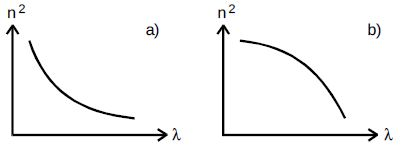
\includegraphics[width = 8cm]{img/dispersion.JPG}
		\caption{Gestalt der Dispersionskurven. a) f"ur $\lambda >> \lambda_\mathrm{1}$, b) f"ur $\lambda << \lambda_\mathrm{1}$ \cite{anleitung}.}
		\label{dispersion}
	\end{figure}

	Dies ist der Fall f"ur normale Dispersion, da der Brechungsindex mit zunehmender Wellenl"ange sinkt. Bei Anomaler Dispersion w"are es der umgekehrte Fall und der Brechungsindex w"urde zunehmen. Dies wird in der N"ahe von Absorptionsstellen $\lambda_\mathrm{i}$ beobachtet. Eine Beschreibung ist nicht durch die Gleichungen \ref{eqn:dispersion1} und \ref{eqn:dispersion2} m"oglich.

	\subsection{Abbesche Zahl} % (fold)
	\label{sub:abbesche_zahl}

	Die Abbesche Zahl ist eine weitere wichtige Gr"o"se in der Optik. Je kleiner die Zahl ist, umso gr"o"ser ist die Dispersion. Sie stellt damit eine grobe Klassifizierung von Glassorten da. Daher wird sie f"ur die Konstkruktion einfacher Linsensysteme verwendet, um deren Aberration zu verringern. 

	Es gilt:

	\begin{equation}
		v = \frac{n_\mathrm{D} - 1}{n_\mathrm{F} - n_\mathrm{C}} \label{eqn:abbe}
	\end{equation}

	Die Gr"o"sen $n_\mathrm{D}$, $n_\mathrm{F}$ und $n_\mathrm{C}$ stellen die Brechungsindices f"ur die Wellenl"angen der Frauenhoferschen Linien dar: $\lambda_\mathrm{C} = \SI{656}{\nano\meter}$, $\lambda_\mathrm{D} = \SI{589}{\nano\meter}$ und $\lambda_\mathrm{F} = \SI{486}{\nano\meter}$.

	\subsection{Aufl"osungsverm"ogen eines Prismen-Spektralapparates} % (fold)
	\label{sub:aufl_osungsverm_ogen_eines_prismen_spektralapparates}
	
	Das Aufl"osungsverm"ogen gibt an, wie gering der Wellenl"angenunterschied $\Delta\lambda$ zweier benachbarter Spektrallinien werden darf, sodass sie vom Ger"at gerade noch getrent werden k"onnen.

	Es ergibt sich der Ausdruck \eqref{gl:aufloesung} f"ur das Aufl"oseverm"ogen A.

	\begin{equation}
		A := \frac{\lambda}{\Delta\lambda} \label{gl:aufloesung}
	\end{equation}

	Dabei ist $\lambda$ die gemittelte Wellenl"ange der beiden Spektrallinien.

	\begin{figure}[!h]
		\centering
		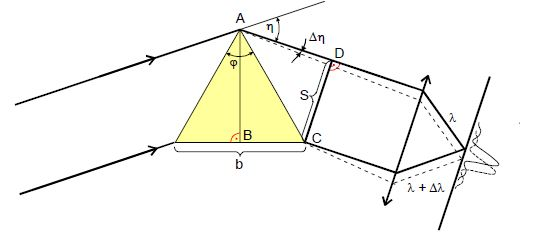
\includegraphics[width = 10cm]{img/aufloesung.JPG}
		\caption{Skizze zum Aufl"osungsverm"ogen eines Prismenspektralapparates \cite{anleitung}.}
		\label{fg:aufloesung}
	\end{figure}

	Fallen zwei Spektrallinien mit den Wellenl"angen $\lambda$ und $\lambda + \Delta\lambda$ in das Prisma, werden sie in leicht unterschiedliche Richtungen gebrochen.
	Eine Trennung der beiden Linien soll genau dann noch m"oglich sein, wenn das Helligkeitsmaximum der einen gerade in das erste Minium der anderen f"allt.

	F"ur die Dispersion des Glasmaterials gilt nach Kapitel \ref{sub:beschreibung_der_messapparatur} Gl. \eqref{eqn:brechungsindex}:

	\begin{equation}
		n(\lambda) = \frac{\sin( \frac{\eta + \varphi}{2} )}{\sin(\frac{\varphi}{2})} 
	\end{equation}

	Wird hier nun $\lambda + \Delta\lambda$ eingesetzt, ergibt sich:

	\begin{equation}
		n(\lambda + \Delta\lambda) = n(\lambda) + \Delta\lambda \frac{\mathrm{d}n}{\mathrm{d}\lambda}	\frac{\sin( \frac{\eta + \Delta\eta + \varphi}{2} )}{\sin(\frac{\varphi}{2})}  \label{disp lambda}
	\end{equation}

	Mithilfe der N"aherungen $\cos(\frac{\Delta\eta}{2} \approx 1)$, $\sin(\frac{\Delta\eta}{2}) \approx \frac{\Delta\eta}{2}$ und $\Delta\eta = \frac{\lambda}{s}$ l"asst sich Gl. \eqref{disp lambda} umformen zu:

	\begin{equation}
		\frac{\lambda}{\Delta\lambda} = 2s \frac{\mathrm{d}n}{\mathrm{d}\lambda} \frac{\sin(\frac{\varphi}{2})}{\cos(\frac{\eta+\varphi}{2})} \qquad .
	\end{equation}

	Mithilfe der Winkelbeziehungen aus Grafik \ref{fg:aufloesung} aus den Dreiecken ABC und ACD ergibt sich f"ur das Aufl"osungsverm"ogen:

	\begin{equation}
		\frac{\lambda}{\Delta\lambda} = b \frac{\mathrm{d}n}{\mathrm{d}\lambda} 
	\end{equation}